\chapter{Client Side}

\section{AngularJS, a bit of background}
\paragraph{}
To understand the structure of WebSlicer a few things must be known about how AngularJS applications are structured and a bit about how AngularJS itself works.
\cite{meding-2016}, has more detailed explanations of each angular componenet than those that follow should the reader need more detail than that provided.
\subsection{Controllers \& Data Binding}
% talk about digest cycle here
\paragraph{}
% use my paper about all of these items to paraphrase.

\subsection{Factories \& Services}
\paragraph{}
\subsection{Directives}
\paragraph{}

\section{WebSlicer AngularJS Structure}
% Talk about my specific implementation. Especially the structure.
\paragraph{}%app.js
The AngularJS structure of WebSlicer is shown in Figure \ref{fig:client-side-structure}.
Flow through this diagram starts with the app.js node which represents the main controller of the application.
This can be thought of as a main function in C++.
The main control variables are also inside of app.js which are similar to global variables.
Variables in this controller are used to store the current settings, file pointer, and output gcode.

\paragraph{}%index.html
Figure \ref{fig:client-side-structure} also shows that index.html is large hub and as WebSlicer is a single page web application this is the only static HTML file.
Index.html has several other functions such as bringing in all libraries and including the custom directives.



% this figure describes my full angular structure on the client
\begin{figure}[!ht]
  \centering
  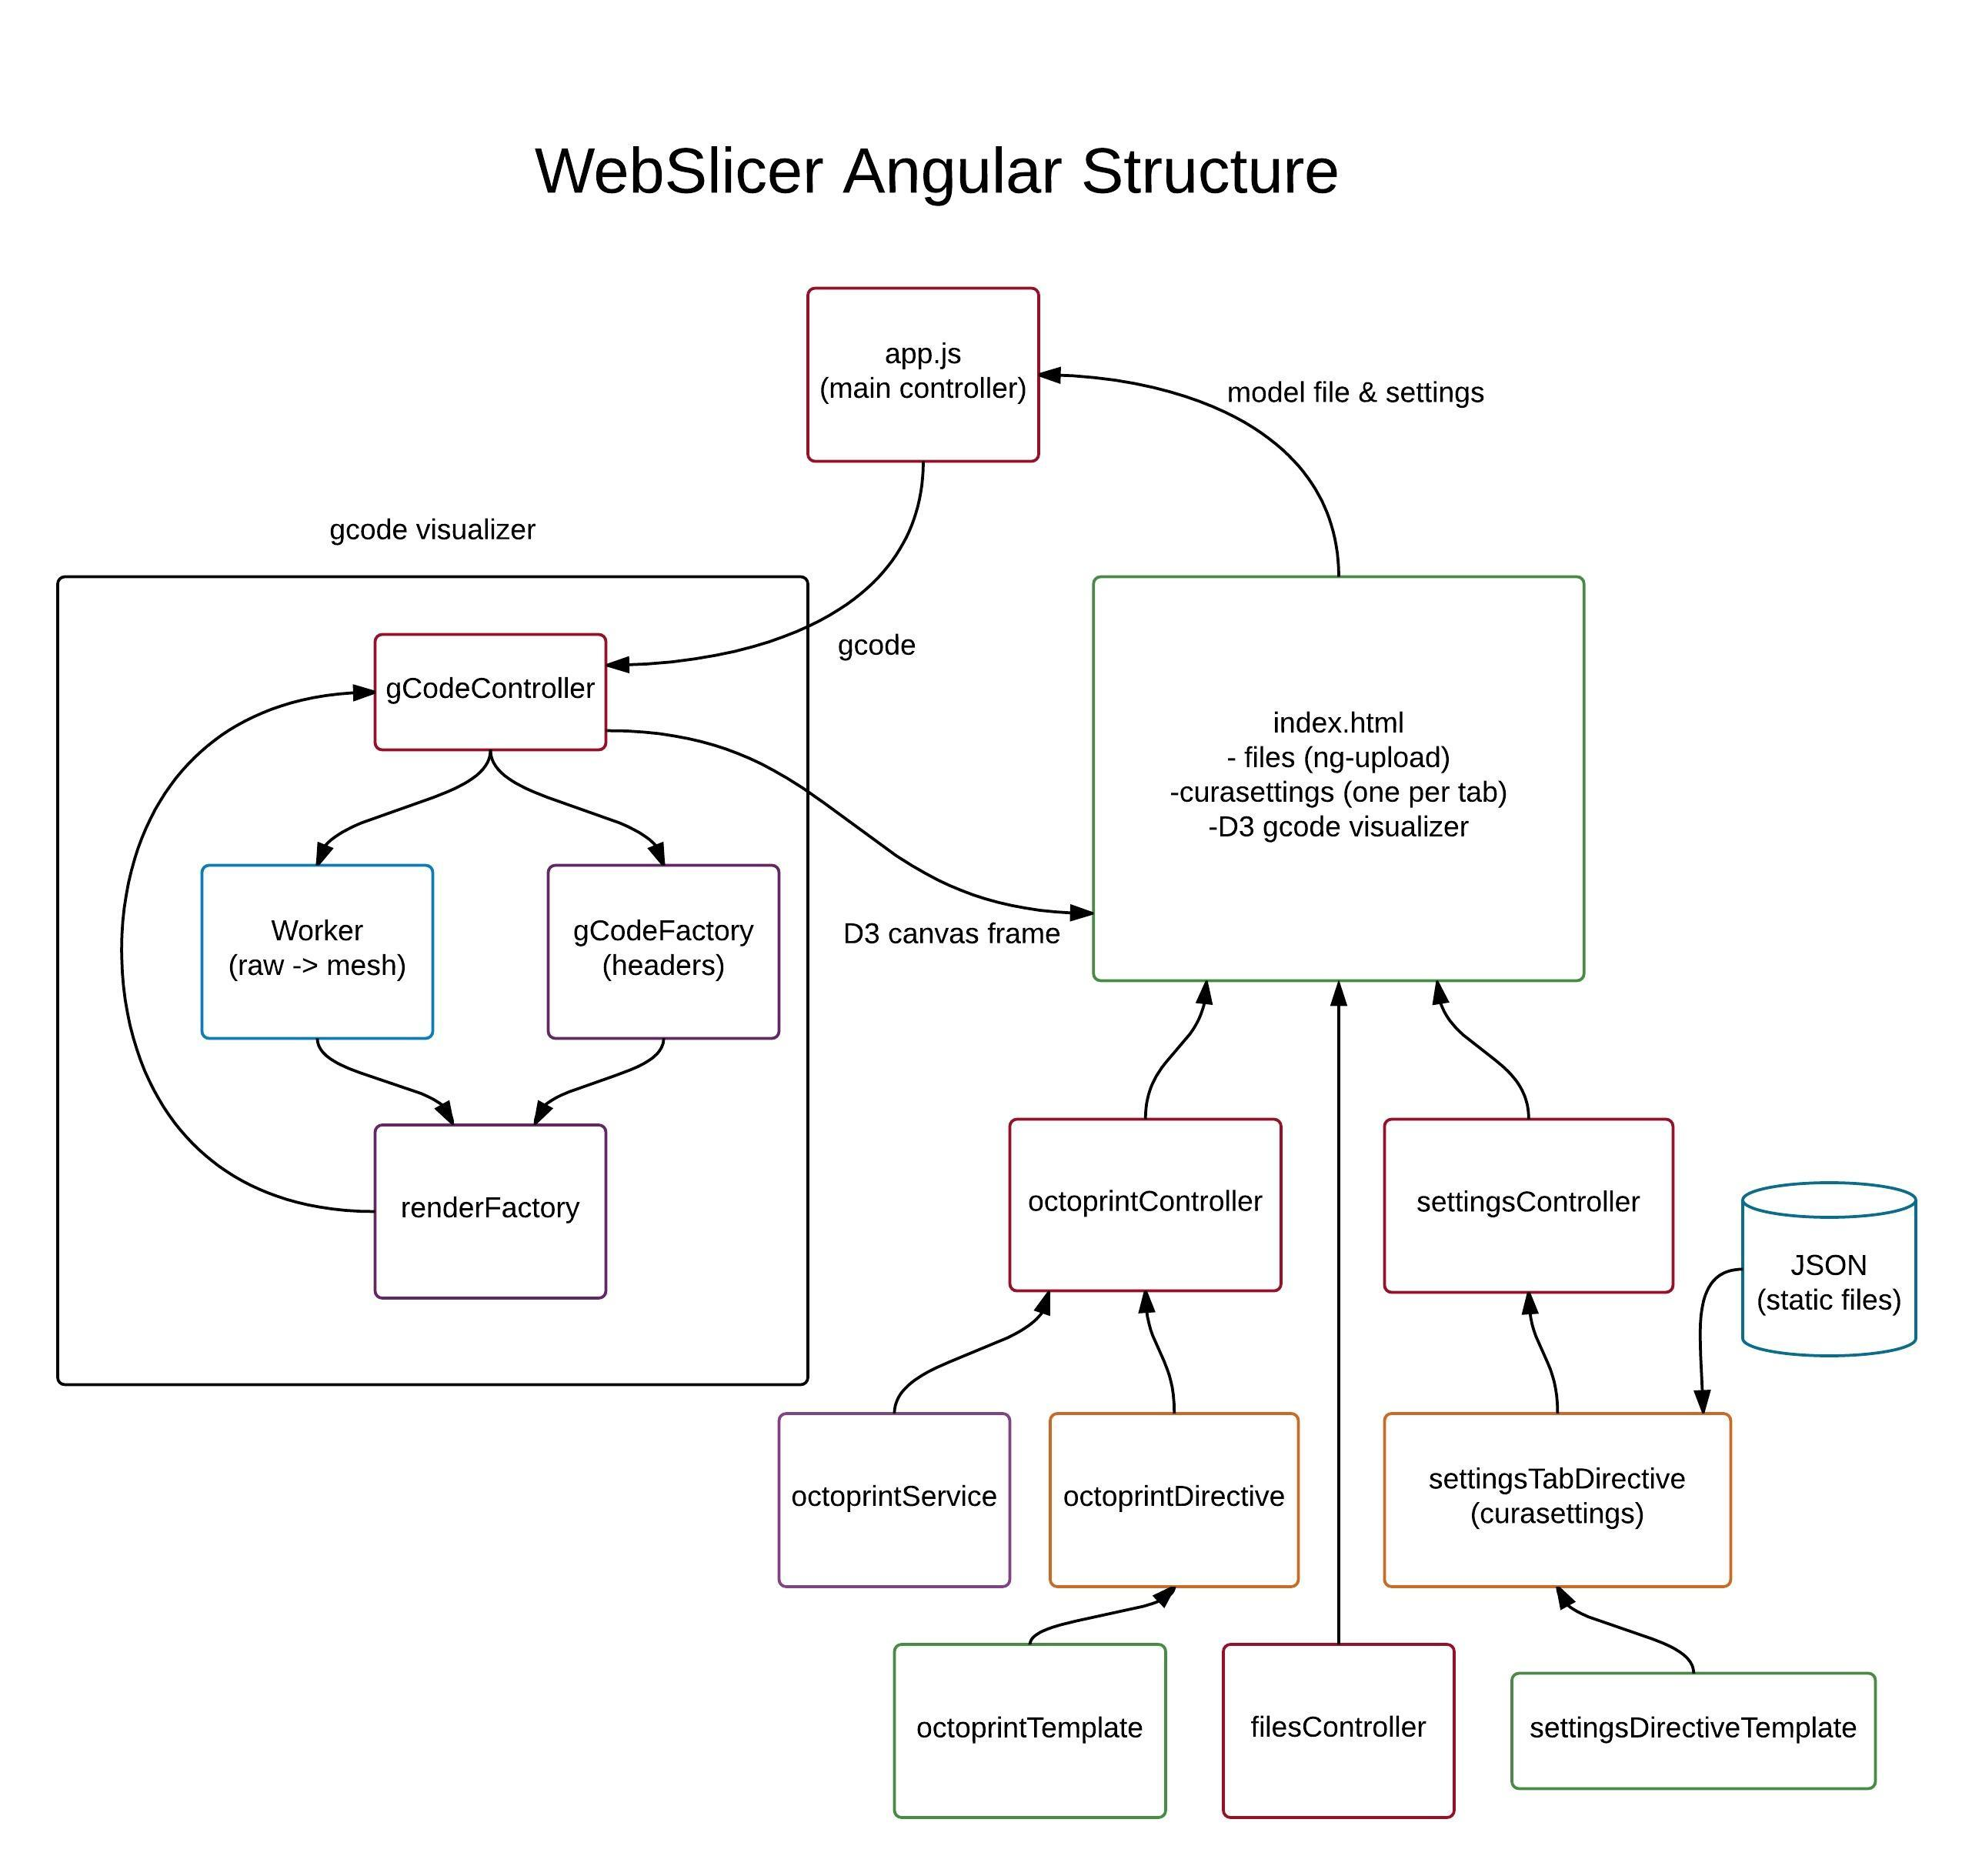
\includegraphics[width=\linewidth]{Client-Side-Structure}
  \caption{Full AngularJS structure breakdown}
  \label{fig:client-side-structure}
\end{figure}

\section{Settings Flow}
\paragraph{}

% TODO: describe this diagram better
\begin{figure}[!ht]
  \centering
  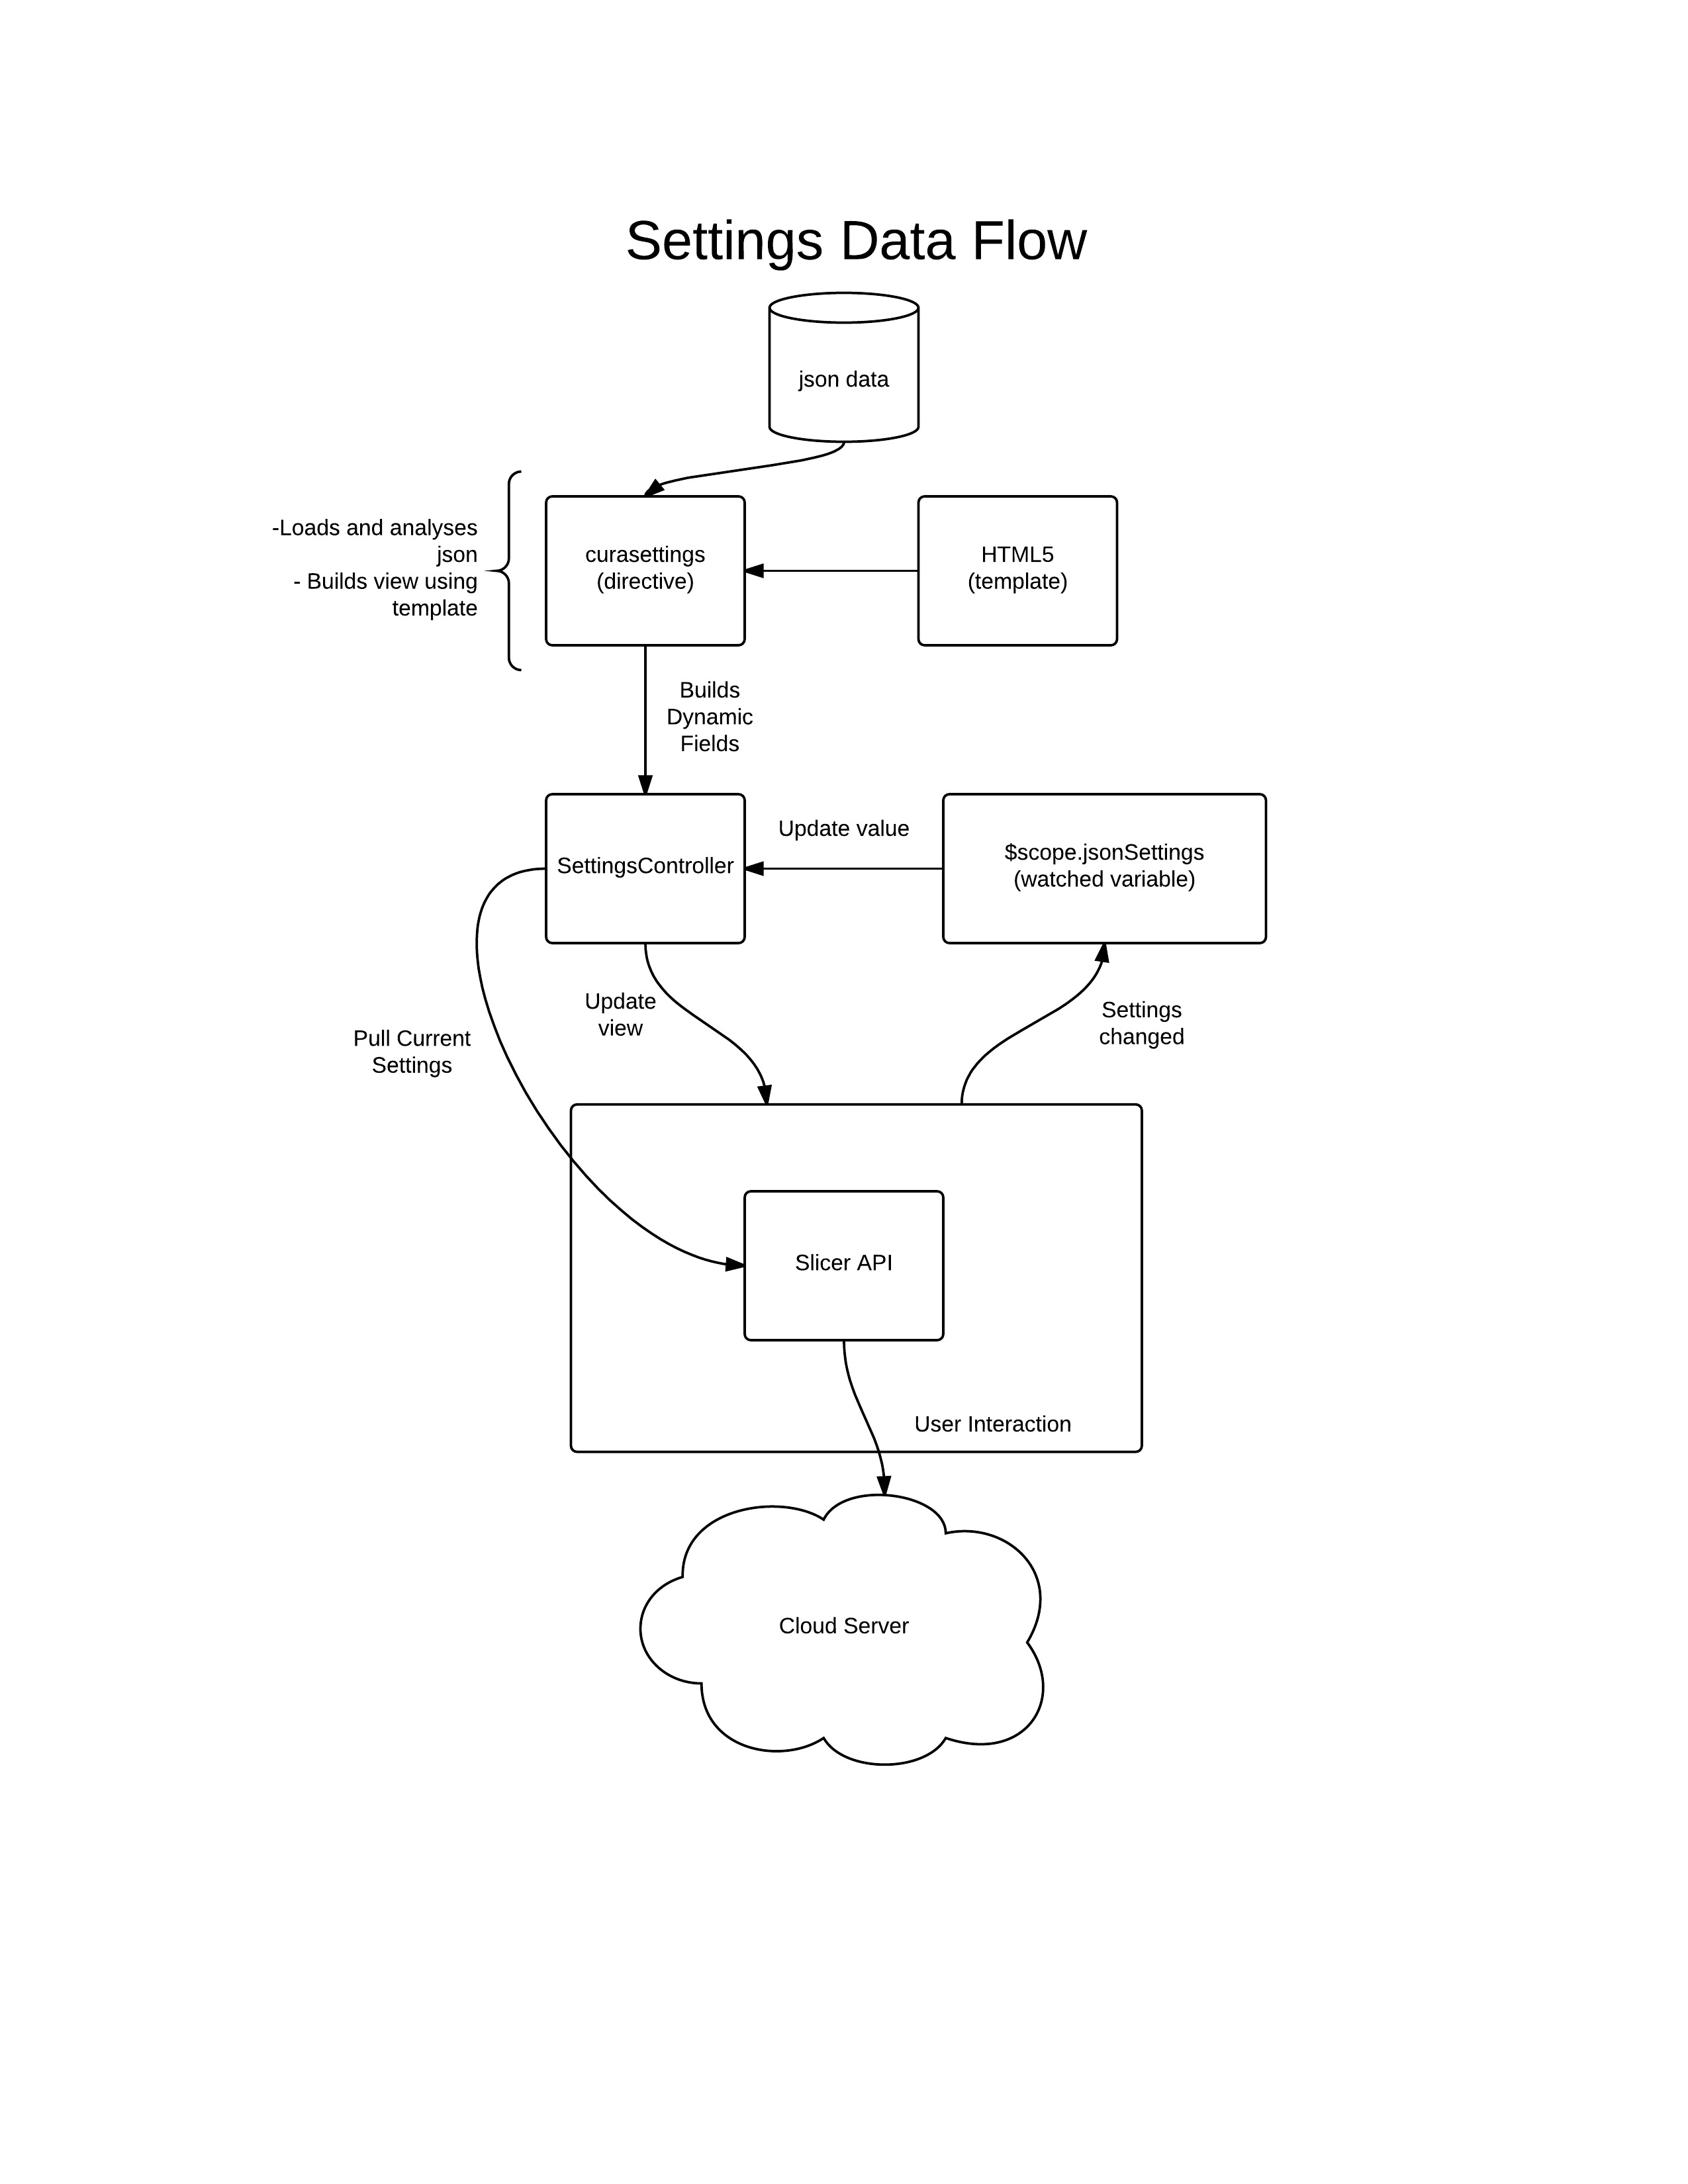
\includegraphics[width=\linewidth]{Settings-Data-Flow}
  \caption{The flow of data through the application from beginning to end of client side user interaction}
  \label{fig:settings-data-flow}
\end{figure}

% TODO: describe settings code and how it works in far more detail
\paragraph{}
As shown in Figure \ref{fig:settings-data-flow}, the client side of this applicaiton has a lengthy flow of data.
This data flow starts with loading a static JSON (JavaScript Object Notation) file which describes the settings in a pattern as shown in Listing \ref{lst:json-settings}.

% JSON settings example listing
\begin{lstlisting}[language=json, label={lst:json-settings}, caption=A sample from a static settings file in JSON format.]
{
    "setting": "layer_height",
    "default": 0.1,
    "type": "float",
    "category": "Quality",
    "label": "Layer Height (mm)",
    "description": "Layer height in millimeters. This is the most important setting to determine the quality of your print. Normal quality prints are 0.1mm, high quality is 0.06mm. You can go up to 0.25mm."
}
\end{lstlisting}

A directive called curasettings takes this static JSON file and splits it up so that for each setting object a field can exist in the template.
AngularJS provides this functionality through the use of an ng-repeat which is written in a similar fashion to that of a for loop in Python.

%TODO: include listing of sample ng-repeat from template.
%TODO: talk about data binding with settings object

\section{Key Challenges}
\subsection{Visualizer Integration}
\paragraph{}
%talk about original design vs final design
%what does the web worker do?
\subsection{Interpolating Settings}
\paragraph{}
%talk about having to get in contact with ultimaker development team about how settings worked


\section{Other Planned Integrations}
%thingiverse / youmagine

\section{Issues \& Known Bugs}
%minimum viable product.
%no login
%display gcode crashes browser
%no 3D view of model

